\documentclass[letterpaper,11pt,leqno]{article}
\usepackage{paper}
\bibliographystyle{bibliography}

% PDF metadata and paths
\hypersetup{pdftitle={How Informative are Job Posting Skill Measures? Evidence from Selection Decisions}}

\begin{document}

% Title and authors
\title{How Informative are Job Posting Skill Measures? \\ Evidence from Selection Decisions}
\author{%
 Nikhil George \and Ramayya Krishnan \and Rahul Telang%
 \thanks{The authors are at Carnegie Mellon University. We gratefully acknowledge support from the Block Center for Technology and Society at Carnegie Mellon University. We thank our partner firm for their collaboration and valuable data access. We also appreciate the helpful feedback received from conference and seminar participants. The analysis and conclusions presented in this paper are those of the authors.}%
}
\date{December 2024}

\begin{titlepage}
\maketitle

Information in job postings plays an increasingly central role in modern labor markets; aside from information for 
potential employees the content in them is a key part of matching algorithms, screening tools, and broader workforce 
analytics. This brings up the demand to ascertain how the measures of skills and job requirements built from job postings 
predict actual selection outcomes. We provide a first validation of the informativeness by predicting selection to internal 
jobs at a major firm from a measure of skill distance built on job postings. Skill distances built on job postings 
strongly predict selection - the probability of selection is 84\% higher when the sought job is in the lowest quintile 
of skill distance compared to a position in the highest distance quintile. And in 70\% of cases the selected candidate 
is the one with the shortest skill distance. These skill measures consistently outperform traditional employee 
characteristics in explaining selection. We build on this validation to show how internal application intensity is 
strongly correlated with average skill distance to emerging opportunities - novel insights relevant to human capital 
management and research on employee mobility in modern labor markets. Beyond validating posting informativeness through 
selection outcomes, our analysis reveals rich possibilities for research and analytics leveraging the skill content 
in job postings.

\end{titlepage}

% Main sections

\section{Introduction}


Major corporations like Google, Walmart, and IBM, along with other public and private agencies, have committed to 
skills-based hiring policies, focusing on capabilities rather than traditional credentials such as degrees or work 
experience \citep{hbr2022skillsbased, mckinsey2020future, wef2020jobs}. This shift comes at a time when employees 
increasingly pursue less fixed career paths both within and across firms, and when the skills required to perform 
modern work evolve rapidly. These forces compel firms to articulate skill requirements and job responsibilities 
with greater precision in their postings. This information is not only consumed by potential applicants—it is 
embedded in the algorithms used by platforms like Indeed and LinkedIn to curate and match opportunities to 
candidates, and ingested by sophisticated screening tools that shortlist applicant resumes based on fit against 
these requirements. Job postings and their content are also systematically harvested by specialized firms like 
Revelio and Lightcast, who package this data into analytical products that provide insights into workforce skill 
requirements across industries\footnote{The workforce analytics provided by firms like Revelio and Lightcast have 
not only supported businesses but also spurred a growing body of academic research that study trends in skill 
demands and job creation \citep{goldfarb2020artificial, azar2020concentration}, and other critical labor market 
phenomena \citep{hershbein2018recessions, forsythe2020labor, braxton2023technological}.}. These developments 
underscore the growing importance of job postings as a key source of valuable information at the analytical, 
strategic, and policy levels.

Despite this growing centrality of job posting content and significant investment in its analysis, no rigorous validation 
exists of whether posting-derived skill measures predict actual selection and mobility outcomes. While firms are 
investing in more detailed skill descriptions, and sophisticated tools are being built to extract and analyze this content, 
consumers of posting-based analytics and tools operate without clear evidence of informativeness. Legitimate concerns 
exist - postings might be aspirational rather than realistic, could be template-driven or overly generic, and might 
list ``nice to have" skills rather than true requirements. Understanding how informative these postings are for 
measuring skill requirements is crucial for the growing ecosystem of tools and analytics being built on this content. 
The ability to validate posting-derived measures against selection decisions would inform both current applications 
and future innovations.

We partner with the IT division of a major financial services firm to study the informativeness of job postings by 
linking it to actual workers and their mobility process. This setting provides an ideal laboratory - the firm's 
hiring process generates detailed position requirements through job postings, which multiple internal candidates 
consider and apply to. The firm's internal job board offers comprehensive records of both successful and unsuccessful 
applications over multiple years. Crucially, we can link the applicants to the postings of their current job and 
observe both successful and unsuccessful applications, providing the opportunity to assess the informative content 
in job postings to predict selection. By structuring a prediction problem, we can examine whether the skill 
distances derived from posting content meaningfully predict selection outcomes, thereby contributing a first of 
its kind estimate of the nature and level of informativeness in job postings; an information source of increasing 
application inside and outside the firm.

Our analysis reveals substantial predictive power in posting-derived skill measures. The probability of selection 
decreases by 84\% when comparing applications in the lowest versus highest quintile of skill distance, indicating 
posting content captures meaningful differences in worker-job fit. This predictive power is particularly evident 
when examining vacancies with multiple applicants - in 70\% of these cases, the candidate with the shortest skill 
distance was selected. The predictive relationship holds both across vacancies and within applicants (across their 
different applications). Notably, traditional employee characteristics like age, tenure, and work experience 
contribute minimally beyond the skill distance measure - suggesting the rich information in job postings dominates 
standard observable characteristics in explaining selection outcomes.

The first step in our machine learning pipeline converts the key information in a job posting to a job skill-embedding 
by mapping it in the language space of a pre-trained language model. While these embeddings capture rich semantic 
relationships in general language, our context of technical skills and responsibilities likely lies in a much 
lower dimensional space. Moreover, with relatively few selection decisions compared to the embedding dimensions, 
we need dimension reduction to enable effective learning of the distance metric. The distance metric learning, 
akin to fine-tuning the general language model's notion of similarity for our specific context, reveals meaningful 
skill relationships. This learned representation's validity is demonstrated through its strong predictive power on 
held-out selection decisions, and its application reveals novel patterns in how employees navigate opportunities 
based on skill-fit.

We apply the skill distance measure to investigate internal job application patterns, revealing another dimension of 
job posting informativeness. Those whose skills closely match available vacancies adopt a relatively passive approach 
despite higher chances of success, while employees facing larger skill distances actively pursue positions requiring 
skill development. By structuring standard posting and mobility data, we show how posting-derived analytics can generate 
actionable insights about whether reducing search frictions or investing in skill development should be prioritized. 
Such capabilities suggest a promising direction for HR analytics, a field that has seen limited advancement despite 
significant interest \citep{Tambe2019} - the combination of skill information in job postings and mobility patterns 
enables rich workforce analytics. Our analysis reveals novel patterns about internal mobility, providing evidence 
about job search behavior in an environment characterized by employed workers navigating evolving skill requirements 
- a setting distinct from traditional unemployment-focused search models. This ability to measure skill requirements 
from job postings and track mobility decisions opens new possibilities for personnel economics research to 
systematically investigate career navigation and skill development choices.

Our paper illuminates the informative content in job postings by linking their skill and responsibility descriptions 
to selection outcomes and application decisions. Through selection prediction, we provide first validation that 
posting-derived skill measures capture meaningful differences in worker-job fit - a crucial validation given the 
growing use of posting content in platforms, analytics, and research. Through our inquiry into application patterns, 
we illuminate how this posting information relates to mobility behavior. This analysis demonstrates significant 
potential for firms to gain insights about internal mobility and its relationship to skill-fit by leveraging 
posting information, while opening new research possibilities in understanding how employees navigate careers 
in environments characterized by evolving skill requirements.

To summarize, this paper illuminates how findings validate a fundamental data source driving major market decisions 
while demonstrating rich analytical possibilities. By showing posting content contains meaningful skill information 
that predicts outcomes, we inform the growing ecosystem of screening tools and analytics built on this content. The 
results challenge pessimism about HR analytics by showing how posting information can guide specific 
interventions - from reducing search frictions for well-matched workers to targeting skill development where needed. 
This posting-based approach outperforms traditional collaborative filtering methods by leveraging the rich content 
in job descriptions, opening new avenues for research in labor economics and personnel practices.

\subsection{Literature Review}

Our work advances a rich technical literature on job recommendation, worker-job matching, and skill 
representation learning---supporting platforms that facilitate job search, candidate-opening matching, and 
career trajectory modeling\footnote{The technical literature has included work on recommender systems 
\citep{shaha2012survey,siting2012job} and representation learning \citep{heap2014combining, zhu2018person, 
liu2019tripartite, bian2020learning} to support platforms facilitating job search 
\citep{heap2014combining,giabelli2021skills2job}, matching jobs to candidates \citep{zhu2018person,qin2020enhanced} 
and modeling career paths and skill recommendations \citep{maurya2017bayesian, kokkodis2021demand}.}. While these 
advances demonstrate sophisticated ways to process job posting content, their focus on platform functionality leaves 
open the fundamental question of whether derived skill measures predict actual selection outcomes. Our work provides 
the first systematic validation of these measures through observed selection decisions.

Our research contributes directly to the Information Systems literature studying algorithms that match workers to 
jobs and recommend skill development \citep{kokkodis2021demand, kokkodis2023good}, while addressing fundamental 
questions about assessing the value of data for algorithmic applications \citep{lei2024value}. Particularly relevant 
is \citet{raghavan2020mitigating}'s documentation of limited transparency in automated screening systems. By 
demonstrating that posting-derived skill measures strongly predict selection, we provide both validation of these 
measures and a framework for evaluating hiring algorithms in practice.

Our work enriches the study of internal labor markets, where different approaches to measuring employee-position 
fit have emerged. \citet{devos2024data} develops recommender systems using collaborative filtering based on observed 
transitions and employee features, while \citet{2024_Cowgill} examines team assignment mechanisms using survey-based 
skill scores validated by management. We demonstrate how the rich skill information contained in job postings can 
generate validated measures of fit that complement these approaches, requiring neither extensive mobility histories 
nor expert validation.

We provide crucial validation for a growing literature in management and economics that leverages job posting text 
to study labor market dynamics. Researchers have extracted signals from job descriptions to examine wage premia 
\citep{Bana2021}, analyze technology's impact on skill demands \citep{George2024}, and forecast effects of 
generative AI \citep{eloundou2024gpts, 2024_Acemoglu}. Our demonstration that posting-derived skill measures 
strongly predict selection outcomes provides important validation for this literature's growing use of posting 
text to measure skill requirements.

Our analysis advances research on career moves and incentives in personnel economics, where studies have documented 
patterns in internal moves \citep{bidwell2024stepping} and efficiency gains from internal hiring \citep{bidwell2011paying}. 
This literature spans from early work on career incentives \citep{baker1994internal, baker1994wage} to recent studies 
of internal labor markets \citep{tambe2020paying, huitfeldt2023internal}. By validating posting-derived skill measures 
and showing how they predict both selection and application patterns, we provide new tools for studying modern career 
navigation in environments where skill requirements evolve rapidly.

We proceed as follows: In Section \ref{sec:research_setting}, we describe the research setting, the 
firm, data and the internal mobility process. In Section \ref{sec:objective_approach}, we outline 
the conceptual ideas of the prediction problem. Section \ref{sec:machine_learning_pipeline} presents 
the machine learning pipeline, the algorithms and details of data processing and implementation. In 
Section \ref{sec:evaluation_skill_distance}, we evaluate the effectiveness of the skill distance metric 
in predicting selection outcomes in detail. In Section \ref{sec:internal_mobility_patterns} we apply 
the distance measure to new positions to study application intensity to new positions vary with skill 
fit and concluding in Section \ref{sec:conclusion_discussion}.


% Research Setting Section
\section{Research Setting}\label{sec:research_setting}

\subsection{Context}

This section outlines our research setting within the Information Technology division of a prominent U.S.-based financial services institution. The division, comprising multiple specialized units, provides technical support ranging from trading systems and wealth management platforms to enterprise-wide initiatives like system modernization and compliance reporting. Several distinctive features make this setting ideal for validating posting informativeness: precise skill specifications required for technical roles, diverse units generating varied requirements, and structured mobility processes yielding both successful and unsuccessful applications.

Within the division, specialized technical roles form the core workforce---application programmers developing trading platforms, data analysts supporting risk management, and quality assurance specialists maintaining enterprise systems. Each position demands specific technical competencies, from programming languages and analytical tools to testing frameworks and development methodologies. Such specialized requirements necessitate detailed articulation of skills in job postings, generating rich content for examining whether posting-derived measures predict selection outcomes.

A centralized job board facilitates internal mobility, where positions are posted with comprehensive skill and responsibility specifications (see Box \ref{box:vacancy_posting} for a representative example). The organization maintains minimal restrictions on internal applications, allowing employees to pursue roles aligned with their interests without prior managerial approval. Following application submission, recruiting units conduct initial screening and interviews to identify suitable internal candidates. External candidates are considered only after a specified timeframe if no appropriate internal candidate emerges.

The organization's structured internal mobility process generates substantial variation in both applications and outcomes across positions. The standardized posting and evaluation procedures, combined with comprehensive data capture of both successful and unsuccessful applications, provide the essential elements for validating posting informativeness through actual selection decisions. This combination of detailed technical postings, standardized processes, and comprehensive outcome data makes the setting particularly suitable for our research objectives.

\subsection{Data}

Our analysis draws on comprehensive data from the firm's Human Resource Information System (HRIS), which captures all job requisitions, applications, and selection outcomes. Each record includes complete job posting content, application details, and final decisions. A crucial feature for our research design lies in our ability to link internal applications to the detailed posting of the applicant's current position at application time, enabling direct comparison of skill requirements between current and sought positions.

\begin{table}[t]
    \caption{Job Postings and Internal Mobility (2018-2021)}
    \begin{tabularx}{\textwidth}{@{}lXXX@{}}
    \toprule
    Year & Total Positions & Internal Applications (\%) & Internal Fills (\%) \\
    \midrule
    2018 & 1,326 & 40.3 & 8.3 \\
    2019 & 1,370 & 50.1 & 17.3 \\
    2020 & 1,606 & 75.7 & 42.5 \\
    2021 & 2,240 & 62.5 & 33.9 \\
    \midrule
    Total & 6,542 & 58.6 & 27.3 \\
    \bottomrule
    \multicolumn{4}{p{\textwidth}}{\footnotesize \textit{Notes:} Data from HRIS covering 2018-2021, supplemented by 1,638 pre-2018 position postings. Internal Applications (\%) represents positions receiving at least one internal application. Internal Fills (\%) represents positions filled by internal candidates.} \\
    \end{tabularx}
    \label{tab:summary}
\end{table}

Table \ref{tab:summary} presents our dataset covering individual contributor positions posted between 2018-2021. The observation window captures 6,542 positions, with 3,836 (58.6\%) receiving internal applications and 1,789 (27.3\%) filled internally. This data is supplemented by 1,638 pre-2018 position postings, enabling broader coverage when analyzing internal applicants' current positions. The data shows a notable increase in internal mobility over the observation period, with the proportion of positions receiving internal applications rising from 40.3\% in 2018 to 62.5\% in 2021.

\begin{table}[t]
    \caption{Structure of HRIS Data}
    \begin{tabular*}{\textwidth}{@{\extracolsep\fill}lllllcc}
    \toprule
    Date & Requisition ID & Job Description & Applicant ID & Employee ID & Internal & Selection \\
    \midrule
    2021-03 & REQ2021-456 & Hadoop Developer & APP-7K89 & EMP-123 & Yes & Selected \\
    2021-03 & REQ2021-456 & Hadoop Developer & APP-7K90 & EMP-124 & Yes & Not Selected \\
    2021-03 & REQ2021-456 & Hadoop Developer & APP-7K91 & -- & No & Not Selected \\
    2021-04 & REQ2021-457 & Data Analyst & APP-7K92 & -- & No & Selected \\
    \vdots & \vdots & \vdots & \vdots & \vdots & \vdots & \vdots \\
    2021-05 & REQ2021-459 & Sr. Developer & APP-7L95 & EMP-127 & Yes & Selected \\
    2021-05 & REQ2021-459 & Sr. Developer & APP-7L96 & -- & No & Not Selected \\
    \vdots & \vdots & \vdots & \vdots & \vdots & \vdots & \vdots \\
    2021-06 & REQ2021-460 & ML Engineer & APP-7M01 & EMP-130 & Yes & Not Selected \\
    \bottomrule
    \multicolumn{7}{p{\textwidth}}{\footnotesize \textit{Notes:} Sample entries from HRIS. Employee ID is populated for internal applicants or when external candidates are selected. Job Description field contains complete posting content (see Box \ref{box:vacancy_posting}) for representative example of full posting content. Internal flag indicates current employee status.} \\
    \end{tabular*}
    \label{tab:hris_structure}
\end{table}

The structure of our HRIS data appears in Table \ref{tab:hris_structure}, which illustrates the comprehensive information available for each application. The system records application timing, position details, applicant information, and selection outcomes. Crucially, for internal applicants, employee identifiers enable linking to their current positions and corresponding job postings. This linkage capability is essential for analyzing how differences between current and sought position requirements relate to selection outcomes.

\noindent \textit{Notes:} This is a sample vacancy posting with information about the firm, the sub-division, location etc. redacted. The posting demonstrates 
the rich content available for analyzing skill requirements and job responsibilities. 

Box \ref{box:vacancy_posting} demonstrates the typical depth of position postings in our dataset. As shown, each posting contains detailed specifications spanning multiple dimensions: role overview, process context, specific responsibilities, and both mandatory and desired skills. This rich content enables precise measurement of skill requirements and job characteristics, providing the foundation for validating posting informativeness.

\begin{table}[t]
    \caption{Sample Job Requisitions and Internal Applications}
    \begin{tabular*}{\textwidth}{@{\extracolsep\fill}llllc}
    \toprule
    Job Requisition No. & Current Position & Position Applied To & Date & Selected \\
    \midrule
    REQ2021-456 & Data Engineer & Hadoop Developer & 2021-03 & Yes \\
    REQ2021-456 & ML Engineer & Hadoop Developer & 2021-03 & No \\
    \vdots & \vdots & \vdots & \vdots & \vdots \\
    REQ2021-458 & Data Analyst & ML Engineer & 2021-04 & Yes \\
    REQ2021-459 & Software Engineer & Sr. Developer & 2021-05 & Yes \\
    \vdots & \vdots & \vdots & \vdots & \vdots \\
    \bottomrule
    \multicolumn{5}{p{\textwidth}}{\footnotesize \textit{Notes:} Derived from HRIS data by linking internal applicants' Employee IDs to their current positions. Both current and applied-to positions contain detailed requirements as shown in Box \ref{box:vacancy_posting}.} \\
    \end{tabular*}
    \label{tab:requisitions}
\end{table}

Table \ref{tab:requisitions} illustrates how we leverage the HRIS data structure to track internal mobility patterns. By linking internal applicants to their current positions through employee identifiers, we can observe both the positions they apply to and detailed requirements of their current roles. Among positions receiving internal applications, we identified 1,370 cases where we could observe the detailed posting of the applicant's current position at application time, forming the core sample for our analysis of posting informativeness.

\clearpage
\begin{tcolorbox}[colback=boxbackground,colframe=boxframe,sharp corners,
title=Sample Job Description,
label=box:vacancy_posting]
\noindent \textbf{Overview}\\
We are one of the world's leading financial institutions ... and risk management products and services.

\noindent \textbf{Process Overview}\\
Build and evolve a consistent Authorized Data Source within Consumer \& Small Business Bank (CSBB) ... both the strategic and tactical analytics needs of the Consumer Bank.

\noindent \textbf{Job Description}\\
Hadoop developer for multiple initiatives. Develop Big Data Strategy and Roadmap for the Enterprise. Experience in Capacity Planning, Cluster Designing and Deployment. Benchmark systems, analyze system bottlenecks, and propose solutions to eliminate them. Develop highly scalable and extensible Big Data platform, which enables collection, storage, modeling, and analysis of massive data sets from numerous channels. Continuously evaluate new technologies, innovate and deliver solution for business-critical applications.

\noindent \textbf{Responsibilities}\\
Assists the team with the design of the architect layer to ensure re-usable metrics and attributes within the reporting layer. Responsible for creating and maintaining necessary documentation (MDR) to ensure audit readiness where necessary. Prototype improvement ideas. Work effectively with the global team. Expected to play technical leadership as an individual contributor. Articulate challenges, propose and drive solutions ...

\noindent \textbf{Mandatory Skills}\\
Extensive knowledge of Hadoop stack and storage technologies HDFS, MapReduce, Yarn, HIVE, sqoop, Impala, spark, flume, kafka and oozie. Extensive Knowledge on Bigdata Enterprise architecture (Cloudera preferred). Experience in No SQL Technologies (Cassandra, Hbase).

\noindent \textbf{Desired Skills}\\
Experience in Real time streaming (Kafka). Experience with Big Data Analytics \& Business Intelligence and Industry standard tools integrated with Hadoop ecosystem. (R, Python). Visual Analytics Tools knowledge (Tableau). Data Integration, Data Security on Hadoop ecosystem. (Kerberos). Awareness or experience with Data Lake with Cloudera ecosystem.

\end{tcolorbox}


The combination of detailed technical postings, comprehensive observation of application outcomes, and our ability to link current and sought positions makes this setting particularly valuable for validating posting informativeness. The rich content in job postings reflects precise skill requirements for technical positions. Moreover, access to both successful and unsuccessful applications enables robust testing of posting content's predictive power. Our unique ability to observe detailed postings for applicants' current positions at the time of application allows direct measurement of skill distances, providing compelling evidence of whether these measures meaningfully predict selection outcomes.

\section{Objective and Approach}\label{sec:objective_approach}

To test whether job postings contain meaningful information about skill requirements, we develop a distance measure between positions based on their posting content. If postings are informative about skills and requirements, this distance should be inversely related to the probability of selection when a person working in one position applies to fill another. In this section, we outline our goal and approach to learning the distance metric and introduce notation before discussing the details in the following section. To build intuition, let us consider the evaluation of a single internal applicant for a position. Let \(j_c\) denote the job description of the internal applicant and \(j_v\) the job description of the vacancy. There is some \(z_i\), a feature vector of the applicant observed in the selection process, which we do not observe. The decision maker assesses a distance \(\delta(j_v, (j_c, z_i))\) and selects the applicant if:
\[
S(j_v, (j_c, z_i)) = 
\begin{cases} 
1, & \text{if } \delta(j_v, (j_c, z_i)) < \tau \\
0, & \text{if } \delta(j_v, (j_c, z_i)) \geq \tau
\end{cases}
\]
Here, \(S\) is a binary selection indicator. We observe the set \(A = \{(j_v, j_c, S)\}\) of past decisions, where \(S\) is the observed selection decision. Although we do not observe the feature vector \(z_i\) available to the decision maker, we use the set \(A\) to verify that the probability of selection \(\text{Pr}(S = 1 \mid x_v, x_c)\) is decreasing in \(d(x_v, x_c)\). Our goal is to find a representation function \(f\) that maps job descriptions \(\{j_i\}\) to a set of vectors \(\{x_i\}\), where \(x_i = f(j_i)\). Each vector \(x_i\) encodes information about the skills and responsibilities described in \(j_i\). We then want to choose an appropriate distance metric \(d(x_v, x_c)\) defined on the set \(\{x_i\}\) such that \(d(x_v, x_c)\) serves as a stand-in for \(\delta(j_v, (j_c, z_i))\). We aim to choose \(f\) and \(d\) so that a classifier predicting whether an applicant is selected for the position they applied for, based on \(d(x_v, x_c)\), has a high Area Under the Receiver Operating Characteristic Curve (AUC).


Success in predicting selection through the skill distance measure would validate that job postings capture meaningful differences in position requirements. Rather than relying on a uniform probability estimate of selection, the ability to generate varying probabilities based on posting content would demonstrate that these descriptions contain valuable and discriminative information about skill fit. If posting content is informative, the distance between job profile vectors should enable us to distinguish between more and less likely selections based purely on the documented position requirements. This would confirm that the detailed skill descriptions in postings meaningfully capture actual job requirements rather than serving as generic templates.


We will now briefly discuss how we approach testing posting informativeness through this prediction task, before presenting a more detailed version in the following section. Our approach involves mapping job descriptions \(\{j_i\}\) to vectors \(\{x_i\}\) so that the distance \(d(x_v, x_c)\) inversely correlates with the probability of selection when a worker in current job \(c\) applies to vacancy \(v\). Two key ideas guide our approach to choosing the representation and distance metric. First, we leverage the language capabilities of a pre-trained transformer-based language model. While the specialized vocabulary used in IT job descriptions could be represented using more classical NLP approaches, the advanced language capabilities of a transformer model offer significant advantages in capturing subtle differences in skill requirements. Second, we utilize our selection and rejection data in a supervised capacity during the selection process for the representation and distance metric. This means we don't merely use the set of internal applications whose outcomes we observe for validation; we also incorporate this data to learn which aspects of posting content are most informative for predicting selection.


\begin{figure} % Use the figure environment for caption and label
    \centering % Center the picture
    \begin{tikzpicture}[node distance=1.2cm, auto, thick, scale= 1, every node/.style={scale= 1}]
        % Styles for the boxes and arrows
        \tikzstyle{box} = [rectangle, draw, text width=2.5cm, text centered, minimum height=1.5cm]
        \tikzstyle{arrow} = [thick,->,>=stealth]
        \tikzstyle{dotted arrow} = [thick,->,>=stealth,dotted]
        % Nodes
        \node[box] (embeddings) {Pre-trained Embeddings};
        \node[box, right=of embeddings] (reduction) {Dimension Reduction};
        \node[box, right=of reduction] (metric) {Distance Metric Learning};
        \node[box, right=of metric] (selection) {Parameter Tuning};
        \node[box, below=0.8cm of selection] (validation) {Validation}; % Reduced distance
        % Arrows
        \draw[arrow] (embeddings) -- (reduction);
        \draw[arrow] (reduction) -- (metric);
        \draw[arrow] (metric) -- (selection);
        \draw[dotted arrow] (selection) to[bend right] node[midway, below] {Adjust based on AUC} (reduction);
        \draw[arrow] (selection) -- (validation); % This arrow is now shorter due to reduced distance
    \end{tikzpicture}
    \caption{Machine Learning Overview} % Add caption inside the figure environment
    \label{fig:ml_pipeline} % Add label for referencing
\end{figure}

\autoref{fig:ml_pipeline} pictorially outlines our broad approach. The first major idea is to leverage the capabilities of a pre-trained language model. We begin with standard pre-processing of job posting texts, then utilize pre-trained embeddings. In our context, embeddings are numerical representations of entire sentences or paragraphs from job descriptions. These embeddings capture the complex language patterns and specialized vocabulary often found in IT job descriptions. This aligns with our use of a pre-trained transformer-based language model, which excels at generating such representations. This approach provides a rich initial representation of the required skills and responsibilities, setting the foundation for our distance metric learning process. Using embeddings allows us to quantify and compare job descriptions more effectively than traditional text-based methods.

The rich and dense embeddings from general-purpose language models are representations in a much larger space. Our goal is to measure distances between these objects, which lie in a smaller subspace. In high dimensions, most points tend to be roughly the same distance apart; as distance measure is important to us, we want to bring down the dimensionality of our representations. A second motivation is our interest in using the selection/rejection data in a supervising framework to learn a distance metric. The core idea is to learn from data a matrix $M$ to re-weight the distance between the respective representations of two job descriptions. As the observations of internal applications are limited, our ability to reweigh the distance measure is affected with high dimensions, in addition to the aforementioned curse of dimensionality problem of distances becoming less meaningful at higher dimensions. We apply dimension reduction techniques to transition the high-dimensional embeddings to more manageable vectors, facilitating more effective distance metric learning while retaining the most relevant information.


The third aspect of our data analytic framework involves using a distance metric that is fine-tuned to our historical selection and rejection data in a supervised capacity. This ensures that the learned metric is tailored to our specific context. The key idea is that differences along features that matter less for selection should weigh less than differences along features that matter more. Metric learning is a well-established idea in machine learning, which we can apply to learn a custom distance between any pair of job representations. This approach allows us to incorporate the valuable information contained in our past hiring decisions directly into our distance measure.

In practice, we must choose the dimensions of our representations carefully. Too few dimensions would not capture the differences between job profiles adequately, while too many would dampen our ability to take advantage of the supervised framework. We can select the optimal dimensionality of the representation via cross-validation. To measure effectiveness, we will utilize the Area Under the Curve (AUC), allowing us to iteratively adjust our approach. This process of validation and adjustment ensures that our distance metric continually improves in its ability to capture the selection patterns within the firm.


This pipeline integrates pre-trained language models, dimensionality reduction, and supervised distance metric learning, making use of historical application and selection data. By actively crafting our representation and distance metric using real selection data, we can test whether job posting content meaningfully captures differences in skill requirements beyond simple text similarity. With this approach, we aim to validate whether postings contain sufficient information to predict selection outcomes, setting the foundation for examining how informative these descriptions are about actual position requirements and worker-job fit.


\section{Machine Learning Pipeline}\label{sec:machine_learning_pipeline}

In this section, we explain the machine learning pipeline that converts vacancy posting text into continuous numerical 
vectors. We leverage the structured nature of job descriptions to extract high-signal information efficiently. Job 
descriptions, despite their length, follow a consistent format. We focus on the easily detectable Mandatory and 
Desired Skills sections, which provide concentrated information about skill and competency requirements. Using the 
Spacy natural language processing library, we parse these sections to extract key technical skills such as programming 
languages (e.g., Java, Asp.Net), web frameworks (e.g., Django), and testing tools (e.g., Selenium).

While knowledge of technologies is important, the Responsibilities section conveys crucial functional aspects of the 
role. These can vary notably even between positions requiring similar technology skills, such as developers, testers, 
and support engineers. The section typically lists tasks to be performed, which might include 'develop big data strategy,' 
'conduct code reviews,' 'engage with stakeholders' or 'application development.' We extract such task descriptions from 
job responsibilities by employing natural language processing techniques. This includes part-of-speech tagging to identify 
action verbs and dependency parsing to locate their direct objects, which are then combined to form concise verb-object 
phrases representing key tasks. By leveraging the structured format and our knowledge of the postings, we effectively 
eliminate low-signal words in the description. In the following subsections, we describe our machine learning pipeline 
which adheres to two key ideas: leveraging capabilities of a pre-trained language model and utilizing past selection 
decisions. 

\subsection{Pre-trained Embeddings}
Here we describe the approach to mapping the extracted text from job postings to the embedding space of 
a pre-trained language model. This section focuses on generating robust embeddings for informativeness 
assessment, rather than achieving state-of-the-art performance on general semantic similarity tasks. 
Prior to embedding, standard pre-processing steps such as lowercasing, stop word removal, and punctuation 
normalization were applied to refine the text.

To create vector representations of the two parts we employ Sentence-BERT (SBERT), a modification of 
the pre-trained BERT network \citep{devlin2018bert}. SBERT is designed to derive semantically meaningful 
sentence embeddings, making it more efficient for comparing longer text strings than BERT embeddings, which 
are typically word vectors, although the BERT word-level embeddings vary with the context, unlike their 
predecessors \citep{reimers-2019-sentence-bert}. SBERT converts text into dense vector representations, 
effectively capturing the semantic meanings and relationships between words. This model is particularly 
suitable for our needs because it is pre-trained and fine-tuned for similarity tasks, ensuring that it 
can generate fixed-size embeddings that are both informative and consistent. The embeddings are generated 
using the SentenceTransformers library (model: paraphrase-MiniLM-L6-v2). By leveraging SBERT, we ensure that 
our embeddings capture the nuanced language used in job postings, which is critical for accurately representing 
the skills and tasks.

For every job posting $j_i$, we have the set of words $j_i^s$ (skills) and $j_i^t$ (tasks) and obtain SBERT 
embeddings $e_i^s$ ($384 \times 1$) and $e_i^t$ ($384 \times 1$) respectively. This separation allows for 
more granular embeddings and a focused semantic representation of each aspect. To evaluate the benefit of 
this separation, we also conducted a baseline experiment where the 'Mandatory Skills,' 'Desired Skills,' 
and 'Responsibilities' sections were concatenated before embedding (referred to as the 'no-split' approach). 
These embeddings encapsulate the semantic content of the job postings, allowing us to compare and analyze 
them effectively. The dual-embedding approach provides a comprehensive view of each position, highlighting 
both the required competencies and the associated responsibilities. This detailed representation forms the 
foundation for developing a robust distance metric that can accurately reflect the similarity between 
job postings, ultimately aiding in the assessment of internal mobility and selection probabilities.


\subsection{Dimension Reduction: A Two-Stage Approach with PCA and Fuzzy C-Means}

Dimension reduction is a critical step in our machine learning pipeline, transforming the initial high-dimensional 
embeddings into a more manageable and informative representation. To achieve this, we employ a deliberate two-stage 
process: Principal Component Analysis (PCA) followed by Fuzzy C-Means (FCM) clustering. This sequential approach 
combines PCA's strength in capturing linear relationships with FCM's ability to model complex, overlapping 
characteristics of job postings.

Our initial step employs Principal Component Analysis (PCA), a well-established technique for reducing the 
dimensionality of high-dimensional data while preserving the most significant variance. The initial 
Sentence-BERT embeddings, for both skills $(e_i^s)$ and tasks $(e_i^t)$, reside in a 384-dimensional space. 
Working directly with this high dimensionality poses challenges for learning a robust and tailored distance metric. 
PCA addresses this by identifying principal components---orthogonal linear combinations of the original features that 
capture maximum variance in the data. By projecting the data onto these top principal components, we effectively 
reduce dimensionality while retaining the most salient linear information and mitigating the impact of noise. 
We apply PCA separately to the skill and task embeddings, recognizing that these represent distinct aspects of 
a job posting with potentially different underlying structures. Retaining the components that explain 90\% of 
the variance reduces the skill embeddings to 49 dimensions $(p_i^s)$ and the task embeddings to 124 dimensions 
$(p_i^t)$. This difference in dimensionality suggests that skill descriptions exhibit more structured patterns, 
likely due to the specific vocabulary used for technical skills compared to the broader language of job 
responsibilities. While PCA effectively captures linear relationships, the potential presence of 
non-linear patterns motivates our subsequent step using Fuzzy C-Means clustering.


Building upon PCA's dimensionality reduction, we employ Fuzzy C-Means (FCM) clustering to create a representation 
capturing non-linear relationships and allowing nuanced characterization of job postings. Unlike traditional 
clustering methods where each posting belongs to a single cluster, FCM enables membership in multiple clusters 
with varying degrees of association. For example, a posting for a "Senior Java Developer" position might show 
70\% membership in a "Java" cluster, 15\% in "Cloud Technologies," and 10\% in 
"Backend," while having minimal membership in clusters representing "Networking" 
or "QA/QC." Similarly, a "Network Administrator" posting might demonstrate strong membership in 
"Network Infrastructure," moderate membership in "System Administration," and 
lower membership in "Security Protocols," with negligible association to software development clusters. 
These membership probabilities, ranging from 0 to 1, provide a nuanced representation of each position's 
skill and task composition. FCM identifies cluster centers in the PCA-reduced data that represent 
prototypical skill and task profiles, then assigns membership probabilities based on proximity to these centers.

In this dimension reduction step, FCM transforms the PCA-reduced embeddings into vectors of membership probabilities. 
We apply FCM separately to the PCA-reduced skill embeddings $(p_i^s)$ and task embeddings $(p_i^t)$. For skills, 
FCM identifies $k_s$ clusters, representing each job posting with a membership probability vector $(m_i^s)$ of 
dimension $k_s$. Each element represents the posting's alignment with a specific skill cluster---higher values 
indicating stronger alignment with that cluster's skill profile. Similarly, for tasks, FCM identifies $k_t$ 
clusters, producing a membership probability vector $(m_i^t)$ of dimension $k_t$. Concatenating these vectors 
creates our final reduced-dimensional representation $(x_i)$ of dimension $(k_s + k_t)$. While the precise 
interpretation of individual clusters merits further investigation, this representation effectively captures 
each posting's relationship to prevalent skill and task combinations in our data. This provides a foundation 
for learning a distance metric tailored to our organizational context, enabling meaningful comparisons between 
positions based on their skill and task profiles.


\begin{figure}[htbp]
    \centering
    \begin{tikzpicture}
        % Styles for the squares and arrows
        \tikzset{
            square/.style={
                draw,
                rectangle,
                minimum size= 2cm,
                fill=none,
                align=center
            },
            arrow/.style={
                thick,
                ->,
                >=stealth 
            }
        } 
        % Define initial position and shift for squares
        \def\initpos{0}
        \def\shift{2.75}  % Distance between centers of squares
        % Custom labels for each step in the process
        \def\labelsT{{"j_i^t", "e_i^t", "p_i^t", "m_i^t"}}
        \def\labelsS{{"j_i^s", "e_i^s", "p_i^s", "m_i^s"}}
        % Drawing the squares, split squares, and arrows
        \foreach \i in {0,...,4} {
            % Draw split square for the first four
            \ifnum\i<4
                \node[square] (square\i) at (\initpos+\shift*\i,0) {};
                \draw (square\i.south) -- (square\i.north);
                \node at ([xshift=-0.375cm] square\i.center) {$\pgfmathparse{\labelsT[\i]}\pgfmathresult$};
                \node at ([xshift=0.375cm] square\i.center) {$\pgfmathparse{\labelsS[\i]}\pgfmathresult$};
            \else
                % Draw the unsplit square for the fifth one
                \node[square] (square\i) at (\initpos+\shift*\i,0) {$x_i$};
            \fi
            % Draw arrow to next square
            \ifnum\i>0
                \draw[arrow] (square\the\numexpr\i-1\relax.east) -- (square\i.west);
            \fi
        }
    \end{tikzpicture}
    
    \vspace{1em}
    
    \begin{center}
        \small
        \begin{tabular}{lll}
            \textbf{Notation} & \textbf{Description} & \textbf{Dimensions} \\
            \hline
            $j_i^{t/s}$ & Split to task and skill components of $j_i$ & text \\
            $e_i^{t/s}$ & $\text{SBERT}(j_i^{t/s})$ & $384 \times 1$ \\
            $p_i^{t/s}$ & $\text{PCA}(e_i^{t/s})$  & $124 \times 1$ (tasks), $49 \times 1$ (skills) \\
            $m_i^{t/s}$ & $\text{FuzzyC}(p_i^{t/s})$  & $k_t \times 1$ , $k_s \times 1$  \\
            $x_i$ & $m_i^t \oplus m_i^s$ & $k_t + k_s \times 1$ \\
        \end{tabular}
    \end{center}
    
    \caption{This is a pictorial representation of the vectorization process that captures the information in a job posting to a numerical vector. The table provides a summary of the notation and dimensions used at each step of the process.}
    \label{fig:job-vectorization}
\end{figure}


\subsection{Distance Metric Learning}

Having established a numerical representation of job descriptions through our two-stage dimension reduction, 
we now focus on calibrating a distance metric to effectively capture meaningful differences between positions. 
Our approach combines the rich representations derived from pre-trained language models with historical selection 
decisions as a supervisory signal. These past decisions serve as ground truth, helping us identify which aspects 
of job posting content are truly informative for predicting successful hires. Importantly, we do not inject 
selection outcome information into the job postings themselves; rather, historical data guides our metric 
to emphasize the inherently predictive differences in posting content.

Learning a custom metric offers significant advantages over generic distance measures in assessing job posting 
informativeness. Traditional metrics like Euclidean distance treat all dimensions equally, failing to capture 
the varying importance of different skills and responsibilities in actual hiring decisions. Through metric 
learning, we calibrate the weights of our representation vector $(x_i)$ based on how informatively different 
aspects of posting content differentiated between successful and unsuccessful applications. Consider a 
software development position requiring both core technical skills (e.g., expertise in Mainframe development) 
and general workplace skills (e.g., presentation software proficiency). Our metric learns to emphasize 
substantial differences in core technical requirements, which historically strongly predicted selection outcomes, 
while de-emphasizing variations in general skills that had minimal impact on hiring decisions.

We employ the family of Mahalanobis distances, parameterized by a positive semi-definite matrix $(M)$, where 
dimensions are weighted according to their informativeness in distinguishing successful applications. In the 
diagonal case, where $(M)$ contains only diagonal entries, the distance calculation represents an independent 
scaling of each dimension---stretching those that historically differentiated outcomes and compressing less 
informative ones. When $(M)$ is non-diagonal, it can capture more complex relationships through both scaling 
and rotation of the feature space, revealing subtle but informative patterns in the posting content. Formally, 
we define our distance function as:

\begin{equation}
d(x_v, x_c; M) = \sqrt{(x_v - x_c)^T M (x_v - x_c)}
\end{equation}

where $(x_v)$ represents the vector of the sought vacancy, $(x_c)$ represents the vector of the current job, 
and $(M)$ is our calibrated Mahalanobis matrix.

To calibrate $M$, we utilize a dataset $(A)$ of tuples $((x_v, x_c, S_{v,c}))$, comprising vector representations 
of vacancy and current job descriptions with their corresponding selection outcomes. We employ the Mahalanobis 
Metric for Clustering (MMC) algorithm \citep{Xing2002}, which solves:

\begin{align*}
\text{Maximize:} \quad & \sum_{(v,c): S_{v,c} = 0} d(x_v, x_c; M) \\[1em]
\text{Subject to:} \quad & \sum_{(v,c): S_{v,c} = 1} d(x_v, x_c; M)^2 \leq 1 \\
& M \succeq 0
\end{align*}

This formulation calibrates the metric to distinguish between successful and unsuccessful applications by 
maximizing distances between rejected pairs while maintaining bounded distances for selected pairs. Implementation 
uses Python 3.11 and scikit-learn, leveraging 1,060 observations (75\% of our selection decisions) for training. 
The dimensionality of $(M)$, determined by our FCM clustering parameters, influences the granularity of our 
representation of informative skill and task profiles, which we optimize through parameter tuning as discussed next.


\subsection{Parameter Tuning}

To implement the Mahalanobis Metric for Clustering (MMC) algorithm effectively, we need to determine the 
optimal number of clusters for the Fuzzy C-Means (FCM) step: (k_t) for task embeddings and (k_s) for skill 
embeddings. These parameters directly determine how finely our representation can distinguish between 
different types of job postings. The choice of cluster numbers influences our ability to capture meaningful 
distinctions between positions while avoiding overly granular distinctions that might not generalize well. 
Selecting appropriate values is crucial for creating a representation that effectively captures the 
underlying patterns in our hiring data and leads to the most accurate distance metric for predicting 
selection probabilities.

Utilizing our dataset of 1,370 internal applications and their outcomes (excluding cases where internal 
candidates were rejected in favor of other internal applicants), we employ a rigorous 5-fold cross-validation 
strategy on the application dataset (A). For each fold, we test combinations of (k_s) and (k_t), where 
(k_s, k_t \in {2, 3, ..., 20}), subject to the constraint (k_s + k_t < 25). This constraint serves a 
practical purpose: with limited training data, allowing the dimensionality of the Mahalanobis matrix (M) 
to grow too large risks overfitting and poor generalization. For each combination, we train the MMC algorithm 
on the reduced-dimensional representations derived from the SBERT embeddings and FCM, evaluating performance 
on the held-out fold using the Area Under the Receiver Operating Characteristic Curve (AUC).

Our cross-validation analysis, visualized in Figure \ref{fig:AUC}, reveals that optimal performance 
is achieved with (k_s = 17) skill clusters and (k_t = 3) task clusters, yielding an average AUC of 0.62. 
This substantial imbalance between the number of skill and task clusters—17 versus 3—aligns with our intuition 
about job postings: while technical skills tend to be numerous and specific (e.g., programming languages, 
tools, frameworks), job tasks often fall into broader categories (e.g., development, maintenance, management). 
The data-driven optimization of these parameters ensures our representation captures meaningful patterns while 
maintaining generalizability.

\begin{figure}[htb]
\centering
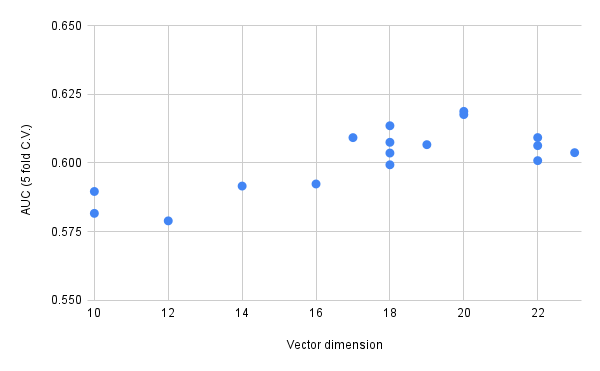
\includegraphics[width=0.75\textwidth]{new_img/chart.png}
\caption{Cross-validated AUC scores across different total dimensionalities (k), showing optimal performance at k = 20}
\label{fig:AUC}
\end{figure}

\subsection{Value of Learning a Custom Distance Metric}

To demonstrate the advantages of learning a distance metric tailored to our organization's selection process, 
we compare our approach against a strong baseline: the cosine distance calculated directly on Sentence-BERT 
embeddings. This comparison helps quantify the value added by our custom metric learning process.

\textbf{SBERT Cosine Distance Baseline:} We established our baseline using the cosine similarity between 
384-dimensional Sentence-BERT embeddings of vacancy and applicant job descriptions. For this baseline, 
we used the 'no-split' approach, concatenating the 'Mandatory Skills,' 'Desired Skills,' and 'Responsibilities' 
sections before embedding. The resulting cosine similarity scores range from -1 to 1, with higher values 
indicating greater semantic overlap between positions. While this approach effectively captures general 
semantic relationships between texts, it treats all aspects of similarity equally, without accounting for 
which differences are most predictive of selection decisions in our specific context.

\textbf{Comparative Analysis:} We evaluated both approaches—the SBERT cosine distance baseline and our 
learned Mahalanobis distance—using the Area Under the Receiver Operating Characteristic Curve (AUC). 
The baseline achieved an AUC of 0.562, indicating some predictive power even with a general semantic 
similarity measure. Our full pipeline, incorporating separate skill and task embeddings with optimal 
cluster parameters ((k_s = 17), (k_t = 3)), achieved a substantially higher AUC of 0.62.

\textbf{Significance of Improvement:} The improvement in AUC from 0.562 (SBERT cosine distance) to 0.62 
(learned Mahalanobis distance) demonstrates the value of our metric learning approach. This gain reflects 
our metric's ability to capture organization-specific patterns in hiring decisions that go beyond general 
semantic similarity. The learned Mahalanobis distance has adapted to recognize which aspects of 
job descriptions are truly predictive of successful hires within our organization. This tailored approach 
leads to more accurate assessments of job fit, with the AUC of 0.62 indicating that our method will 
correctly rank a randomly chosen selected applicant above a randomly chosen rejected applicant 
62\% of the time—a meaningful improvement over both chance (50\%) and the baseline (56.2\%). 
This improvement validates our core premise that job posting text contains valuable information 
about position requirements that can be extracted through careful methodology.

\section{Evaluation: Does Skill Distance Predict Selection?}\label{sec:evaluation_skill_distance}

This section evaluates whether our job postings based skill-distance measure meaningfully captures skill requirements by testing how well 
our derived distance metric predicts selection of internal candidates for new positions. Our primary interest lies in understanding the 
extent to which posting content predicts selection, and in assessing the relative contribution of the skill distance measure compared to 
a few other observed features. While an Area Under the Curve (AUC) of 0.62 might appear modest in a traditional classification setting, 
the key contribution of this section is demonstrating the surprisingly rich and informative signal captured by a distance metric derived 
solely from job posting content. Even with this level of predictive power, we reveal that job postings contain substantial information 
about the skills relevant to selection decisions.

Our test set comprises 308 cases where internal applicants applied to vacancies (approximately 25\% of our total cases). 
We examine whether skill distances computed purely from posting content capture predictable variation in selection outcomes. 
It's important to note that the information contained in an applicant's job description ($j_c$) may not fully capture the skills 
and abilities of that position, let alone those of the candidate. This potential measurement loss informs our approach.
 

\subsection{Skill Distance and Selection Probability}

To assess the relationship between skill distance and selection probability, we employ a logistic regression to quantify the association:

\begin{equation}
\text{logit}(P(\text{S}{c,v} = 1)) = \beta_0 + \beta_1 \times Q_k(d{j_c, j_v})
\end{equation} 

Here, \( Q_k(d_{j_c, j_v}) \) represents the quintile of the skill distance between the applicant's current job (\( j_c \)) and the vacancy (\( j_v \)). We discretize the 
distance into a categorical variable, as the relationship between selection probability and distance is unlikely to be simply linear. This discretization offers stability 
and robustness to extreme values while retaining easy interpretation. \autoref{tab:logistic_regression} shows that the coefficient for skill distance is negative and 
significant \((\beta_1 = -0.3268, \, p < 0.01)\), indicating that applicants with lower skill distance to a vacancy have a higher likelihood of being selected.


\begin{table}[h]
    \centering
    \caption{Logistic Regression Results for Skill Distance and Selection Probability}
    \renewcommand{\arraystretch}{1.2} 
    \begin{tabular}{lcc}
    \hline
    \textbf{Variable} & \textbf{Coefficient} & \textbf{Std. Error} \\
    \hline
    Intercept & 1.1171*** & 0.265 \\
    Quintile & -0.3268*** & 0.086 \\
    \hline
    Observations & \multicolumn{2}{c}{308} \\
    Pseudo R-squared & \multicolumn{2}{c}{0.03551} \\
    \hline
    \multicolumn{3}{l}{\footnotesize{*** p$<$0.01}} \\
    \end{tabular}
    \label{tab:logistic_regression}
\end{table}

The regression suggests that, on average, an applicant-vacancy pair in the lowest skill distance quintile has an 84\% 
higher probability of selection compared to a pair in the highest quintile. This substantial difference in selection 
probability across skill distance quintiles strongly suggests that our posting-derived metric is effectively capturing 
informative variations in the skill alignment between applicants and vacancies.


\begin{figure}[h]
    \centering
    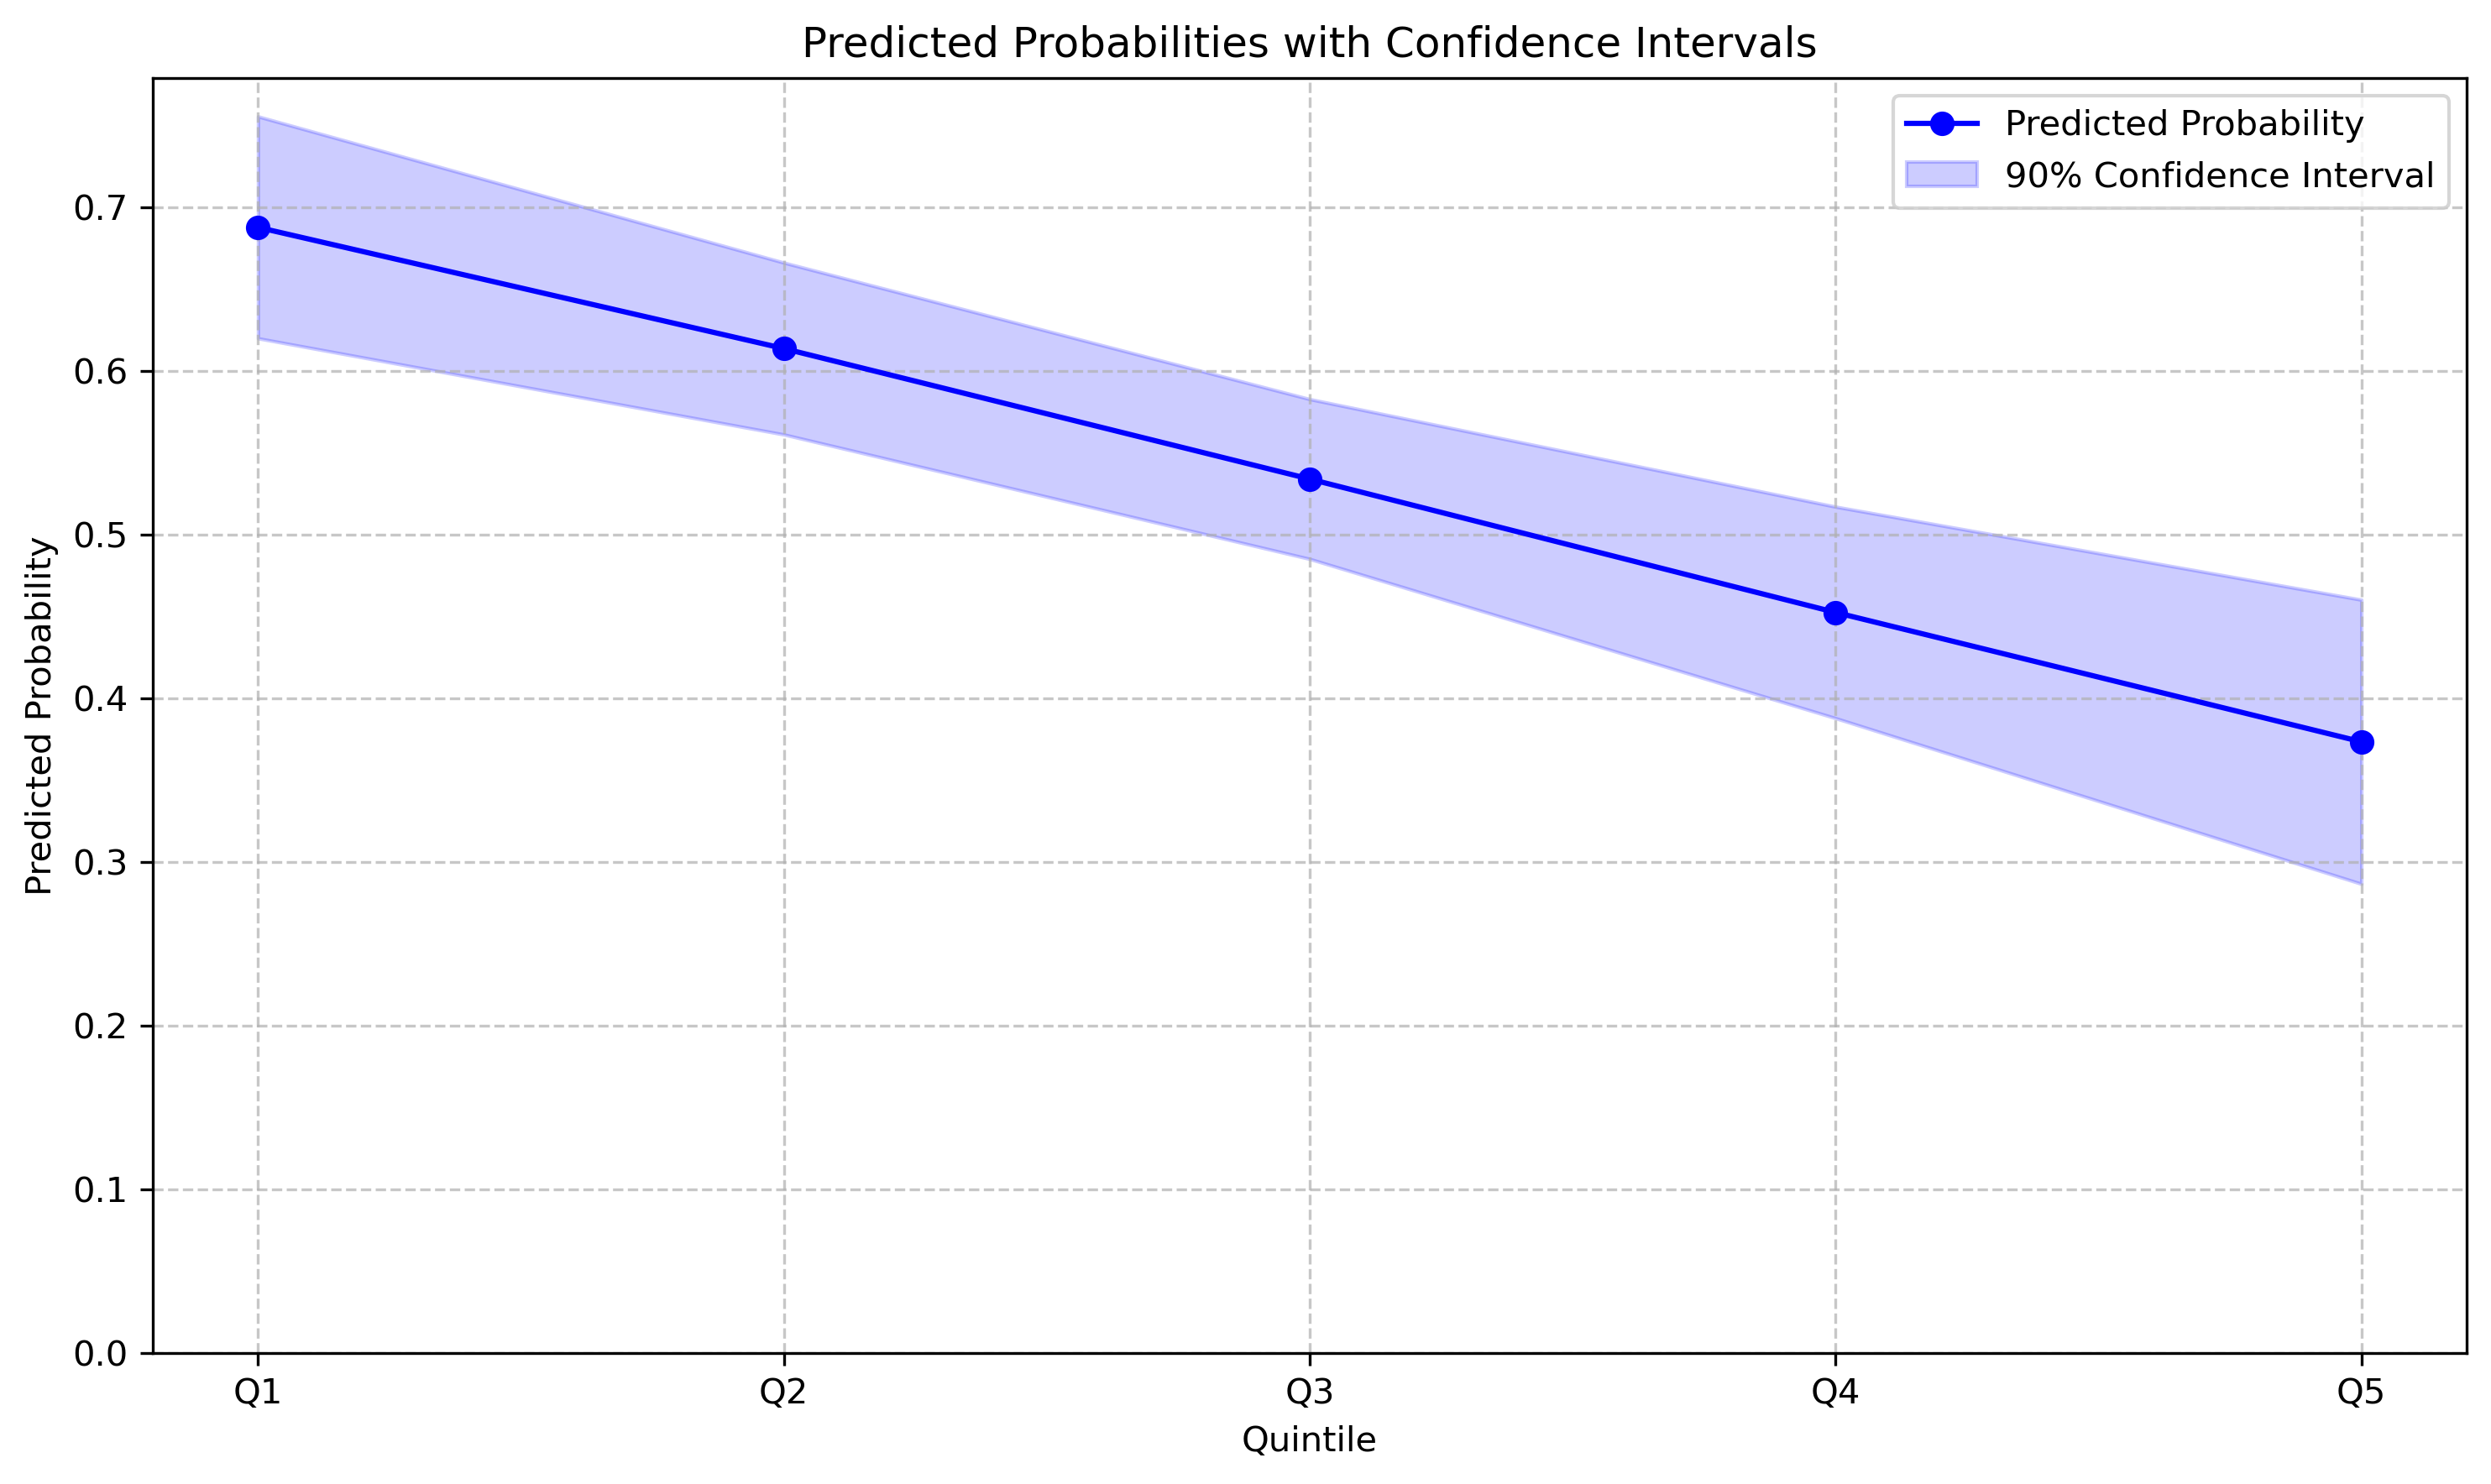
\includegraphics[width=0.75\textwidth]{new_img/pp.png}
    \caption{Selection Probability by Skill Distance Quintile}
    \label{fig:skill_distance_probability}
\end{figure}

While skill distance accounts for a small component of the variation in selection decisions, its ability to capture differences in selection probability is unambiguous. 
We will now exploit the structure in our test sample to examine the association. 


\subsection{Skill Distance: Within-Vacancy and Within-Applicant Variation}

When multiple internal candidates apply to the same vacancy, we have an opportunity to verify if selection among different applicants for the same position is predicted 
by their respective skill distances. Correlation between skill distance and selection measured at each vacancy level would convey a more direct link of the measured distance. 
Similarly, we have cases where an applicant has applied to different vacancies. This allows us to focus on applicant-level selection data to examine whether the applicant 
has a higher selection probability for vacancies to which they have a low skill distance. Focusing on a single applicant allows us to control for unobserved factors that 
influence their selection chances across vacancies, such as broadly relevant skills they have acquired or performance in their current job. While we have already established 
a notable negative association between skill distance and selection, these analyses would further demonstrate that the measured skill distance captures significant selection 
variation at both the applicant and vacancy levels, thereby reinforcing the measure's informativeness.



\subsubsection{Within-Vacancy Selection}

To assess the predictive power of the skill distance metric, we evaluated the proportion of vacancies where the applicant with the lowest skill distance was selected. Our 
analysis encompassed 261 observations across 110 vacancy groups from our test set, each group comprising a vacancy with multiple internal applicants and one selection. The 
analysis revealed that the candidate with the lowest skill distance was chosen in 69.92\% of cases, suggesting the metric's reliability in predicting selection outcomes. We 
further analyzed the role of skill distance in the selection probability among applicants competing for the same vacancy using a conditional logit model. The model incorporated 
vacancy-specific fixed effects ($\alpha_v$) to concentrate on within-vacancy variation. The results indicated that being in a higher skill distance quintile decreased the 
probability of selection by 35\% ($\beta = -0.4293$, $p < 0.01$). The initial exploratory analysis demonstrates the skill distance metric's capacity to predict selection 
outcomes in a majority of cases. Building on this, the more formal conditional logit model enables a rigorous examination of the role of skill distance in differentiating 
applicants within the same vacancy. Together, these findings highlight the relevance and importance of the skill distance measure in the selection process. 

\begin{equation}
\text{logit}(P(\text{S}_{v,c} = 1)) = \alpha_v + \beta Q_k(d_{j_c,j_v})
\end{equation}

\begin{table}[h]
    \centering
    \caption{Conditional Logit Model Results for Within-Vacancy Analysis}
    \renewcommand{\arraystretch}{1.2}
    \begin{tabular}{lcc}
    \hline
    \textbf{Variable} & \textbf{Coefficient} & \textbf{Std. Error} \\
    \hline
    Quintile & -0.4293*** & 0.122 \\
    \hline
    Observations & \multicolumn{2}{c}{261} \\
    Groups & \multicolumn{2}{c}{110} \\
    \hline
    \multicolumn{3}{l}{\footnotesize{*** p$<$0.01}} \\
    \end{tabular}
    \label{tab:within_vacancy}
\end{table}



These results underscore the relevance and importance of the skill distance measure in the selection process. 
Crucially, the ability of skill distance to differentiate between candidates applying for the same position highlights 
the fine-grained informativeness embedded within job postings regarding the specific requirements of that role.

\subsubsection{Within Applicant Selection}

Now, we analyze the ability of our skill distance measure to account for selection decisions within an applicant's multiple vacancies. We again employ a conditional logit model, 
this time incorporating applicant-specific fixed effects ($\alpha_c$).


\begin{equation}
\text{logit}(P(\text{S}_{c,v} = 1)) = \alpha_c + \beta Q_k(d_{j_c,j_v})
\end{equation}

The test dataset now comprises 111 observations from 33 applicant groups, each applying to multiple vacancies. The results reveal that applicants in higher skill distance 
quintiles experience a 50\% reduction in selection probability (\(\beta = -0.695\), \(p = 0.017\)). This demonstrates that the measured skill distance effectively accounts 
for selection decisions within applicants. 


\begin{table}[h]
    \centering
    \caption{Conditional Logit Model Results for Across-Applicant Analysis}
    \renewcommand{\arraystretch}{1.2}
    \begin{tabular}{lcc}
    \hline
    \textbf{Variable} & \textbf{Coefficient} & \textbf{Std. Error} \\
    \hline
    Quintile & -0.695** & 0.290 \\
    \hline
    Observations & \multicolumn{2}{c}{111} \\
    Groups & \multicolumn{2}{c}{33} \\
    \hline
    \multicolumn{3}{l}{\footnotesize{** p$=$0.017}} \\
    \end{tabular}
    \label{tab:across_applicant}
\end{table}


These patterns demonstrate that the skill distance from an applicant's current job provides valuable information for predicting selection to new internal vacancies. While 
selection typically depends on an applicant's skill-set and preparedness for the new position's demands, our findings reveal that a distance measure constructed from job 
postings and past selection decisions correlates strongly with observed selection patterns. This correlation opens an analytical window into the firm, linking skills to 
internal mobility. Before exploring these links we examine how important is the skill distance measure relative to other observed features in predicting selection to vacancies.



\subsection{Other Observed Features}

While our paper primarily focuses on leveraging information from job postings and selection decisions, we recognize the importance of evaluating other predictors of 
internal candidate selection. To enhance our understanding of selection patterns, we examine additional features available in the firm's information system. We compare 
the performance of our skill distance metric against other observed applicant characteristics, including tenure at the organization, total work experience, job category, 
vacancy (job sought) category, and proficiency rating. Table \ref{tab:other_features} presents summary statistics for these features. 

\begin{table}[h]
    \centering
    \caption{Summary Statistics -- Other Observed Features}
    \begin{tabular}{l c c c c}
        \toprule
        \textbf{Notation} & \textbf{Description} & \textbf{Unit} & \textbf{25th Percentile} & \textbf{75th Percentile} \\
        \midrule
        $t_c$ & Tenure at $c$ & days & 661 & 1346 \\
        $T_c$ & Total experience & days & 1927 & 3009 \\
        $l_c$ & Job category & 4 levels & 2 & 3 \\
        $l_v$ & Vacancy category & 4 levels & 2 & 3 \\
        $p_c$ & Proficiency rating & 4 levels & 2 & 2 \\
        \bottomrule
    \end{tabular}
    \label{tab:other_features}
\end{table}

The data shows notable differences among applicants. Tenure ranges from about 2 years to 3.5 years, while total experience spans from roughly 5 years to 8 years at the 25th and 75th percentiles. Job and vacancy categories both range from level 2 to 3, indicating movement across organizational tiers. Proficiency ratings, however, remain consistent at level 2 for at the 25th and 75th percentiles. These observed features, as shown in Table \ref{tab:other_features}, display clear variation across the applicant pool. Their potential to explain selection patterns merits further exploration, complementing our primary skill distance metric.


To assess the relative importance of the skill distance measure  we employ Random Forest classifiers. The well known ensemble learning algorithm captures complex interactions between variables. We train two Random Forest models on our training dataset: one incorporates all features including skill distance, while the other excludes skill distance. This method isolates and quantifies the predictive power of the skill distance metric relative to other observed features. We evaluate these models on our test set and will again employ the AUC metric. Table \ref{tab:model_comparison} presents the AUC scores for both models on the test set.

\begin{table}[h]
    \centering
    \caption{Model Comparison: Random Forest Classifiers with and without Skill Distance}
    \renewcommand{\arraystretch}{1.2} 
    \begin{tabular}{lcc}
    \hline
    \textbf{Model} & \textbf{AUC Score} \\
    \hline
    Full Model (with Skill Distance) & 0.600 \\
    Model without Skill Distance & 0.500 \\
    \hline
    \end{tabular}
    \label{tab:model_comparison}
\end{table}




The full model, which includes skill distance, achieves an AUC of 0.600, while the model without skill distance yields an AUC of 0.500 - equivalent to 
a classifier with no predictive ability. This dramatic difference in performance powerfully illustrates the substantial informative content captured by 
the skill distance measure. Despite the clear variation in other observed features such as tenure, total experience, job categories, and proficiency 
ratings, skill distance alone accounts for nearly all predictable variation in selection outcomes.

This finding is particularly noteworthy given that we derived our measure from job descriptions, which are generally less sensitive than other HR data. 
While firms often possess additional potentially predictive features, these may be subject to privacy concerns or legal restrictions. Our approach demonstrates 
that valuable insights can be derived from less sensitive data sources, advancing the field of people analytics while maintaining ethical data practices. Moreover, 
the granularity of our skill distance measure appears to capture nuanced differences between roles that categorical variables like performance ratings may miss, 
especially when applicants cluster in just one or two groups.

\section{Decoding Internal Mobility Patterns}\label{sec:internal_mobility_patterns}


Having developed a measure of skill distance between positions based on job postings and validating it, we explore how 
this can be applied to understand mobility patterns within the firm. The measure quantifies the distance between skills 
and tasks enumerated in job postings and assesses selection chances of candidates for new vacancies. In this section, 
we apply the skill distance metric to study how internal candidates' application behaviors vary based on their 
prospects at the time of application. By capturing predictable variation in selection, this measure enables a more 
nuanced examination of internal transitions and application patterns. The firm can now pose more sophisticated queries 
about internal mobility. For instance, it can now assess for any employee the proportion of new vacancies where their 
skill distance suggests a high probability of selection based on historical patterns. Central to our empirical 
investigation is the average skill distance measure, which assesses an employee's prospects for movement within the firm. 
From an internal applicant's perspective, if many vacancies share skills similar to their current job, their prospects are 
good; if most vacancies are distant, their prospects are weaker. We first develop this average skill similarity measure, 
then proceed to a detailed empirical analysis of application patterns and internal mobility. This analysis opens up new 
possibilities for understanding and supporting workforce development.




\subsection{Average Skill Distance}

To formalize the concept of average skill distance introduced above, we define the following metric:

\begin{equation}
    \overline{d}_{j_c, t} = \frac{1}{|J_t|} \sum_{j_v \in J_t} d(j_c, j_v)
\end{equation}

where $\overline{d}_{j_c, t}$ represents the average distance to job postings at time $t$, $J_t$ is the set of job postings in time window $t$, and $d(j_c, j_v)$ is the distance between the current job $j_c$ and a vacancy $j_v$. In our empirical analysis, we compute this measure for each internal applicant, considering all vacancies in a 30-day window prior to their observed application. This approach allows us to quantify an employee's prospects at the time of application, as discussed in the preceding paragraph. The distribution of $\overline{d}_{j_c, t}$, illustrated in \autoref{fig:s_dist_hist}, reveals notable heterogeneity in applicants' average skill distances, providing a foundation for our subsequent analysis of application patterns and internal mobility.

\begin{figure}[h]
    \begin{center}
        \begin{minipage}{\textwidth}
            \centering
            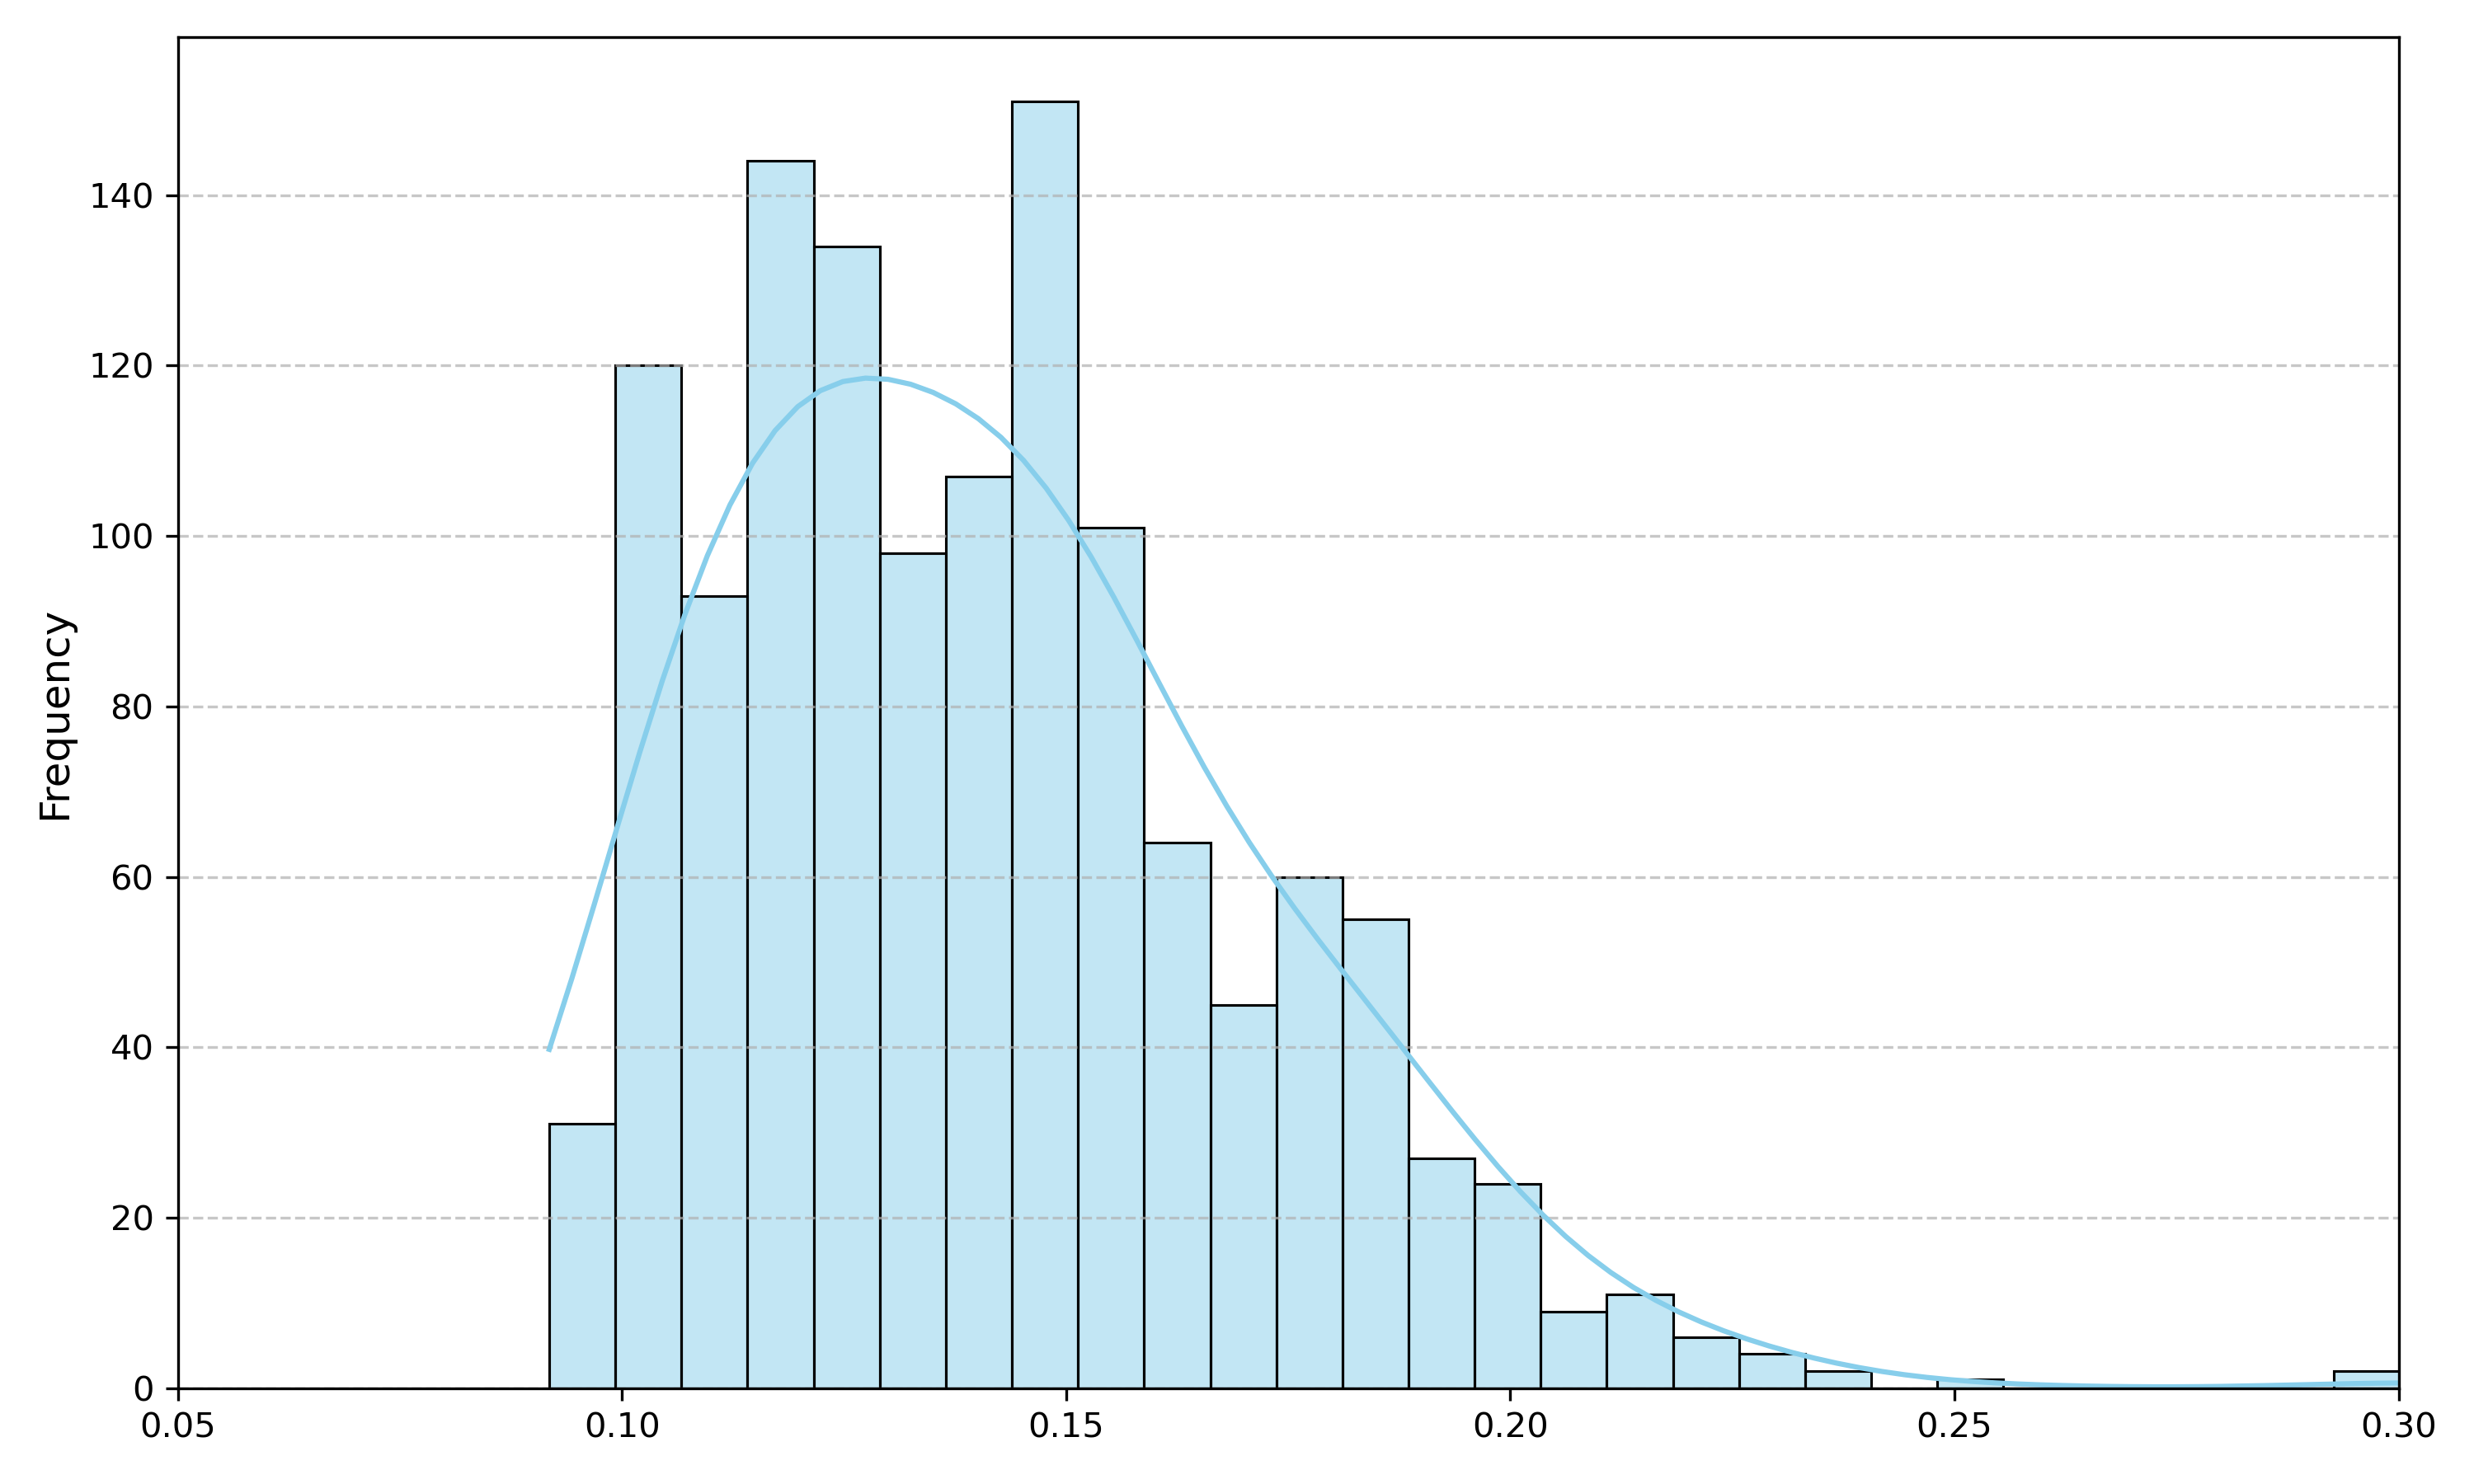
\includegraphics[width=0.8\textwidth,height=0.4\textheight]{new_img/histogram_prosp.png}
            \caption{Distribution of Average Skill Distance (\(\overline{d}_{j_c, t}\))}
            \label{fig:s_dist_hist}
        \end{minipage}
    \end{center}
\end{figure}




\subsection{Empirical Analysis}

Our focus is to develop an understanding of how skill match to vacancies, which we can now measure, affects application 
patterns. Applying is a key step in the internal mobility process and the stage of the search process that can be observed. 
We will look at two aspects of the application process: its directness and intensity. Directness corresponds to whether 
the applicant is applying to positions where they have a higher probability of securing a job, measured using the skill 
distance. Intensity captures how many positions the applicant applies to. Both directedness and intensity improve the 
probability of moving to a new position within the firm. From the firm's perspective, understanding how application 
behavior predictably varies enables them to tweak processes to support employee mobility within the organization. Our 
empirical investigation focuses on three key patterns in application behavior as they relate to the average skill distance 
measure, and we present our findings for each of these patterns in the following sub-sections.


\subsubsection{Average Skill Distance and Application Intensity}

The relationship between an applicant's average skill distance to available vacancies and the positions they choose to 
apply for provides crucial insights into internal mobility patterns. We investigate whether a higher average skill 
distance is associated with applying to closer or farther positions in terms of skill requirements. This analysis 
helps us understand how employees navigate their career paths within the firm when faced with varying degrees of skill 
alignment with available opportunities.

Applicants with a high average skill distance to vacancies face a potentially smaller set of opportunities that closely 
align with their existing skillset. This situation presents a dilemma: do these employees constrain their applications 
to fewer, more closely aligned positions, or do they make more exploratory applications to positions that require 
significant skill development? Conversely, applicants whose skillsets are closer to the available vacancies might 
be less inclined to seek positions that require learning new technologies or skills.

To empirically examine how skill remoteness affects application behavior, we estimate the following model:

\begin{equation}
    d_{j_v, j_c} = \beta_0 + \beta_1 \overline{d}_{j_c, t} + \epsilon
\end{equation}

$d_{j_v, j_c}$ is the standardized skill distance between the current job $j_c$ and the job applied for $j_v$, 
and $\overline{d}_{j_c, t}$ is the standardized average skill distance to vacancies.


\begin{table}[h]
\centering
\caption{Average Skill Distance and Application Intensity} 
\renewcommand{\arraystretch}{1.2}
\begin{tabular}{lcc}
\hline
\textbf{Variable} & \textbf{Coefficient} & \textbf{Std. Error} \\
\hline
Constant & 2.945e-16 & 0.022 \\
$\overline{d}_{j_c, t}$ (std) & 0.6093*** & 0.025 \\
\hline
R-squared & \multicolumn{2}{c}{0.371} \\
\hline
\multicolumn{3}{l}{*** p$<$0.01, ** p$<$0.05, * p$<$0.1} \\
\end{tabular}
\label{tab:skill_remote_app}
\end{table}

The results presented in Table \ref{tab:skill_remote_app} reveal a strong positive association 
between $\overline{d}_{j_c, t}$ and $d_{j_v, j_c}$. Specifically, we find that a one standard deviation 
increase in average skill distance to vacancies is associated with a 0.6093 standard deviation increase 
in the distance to the position applied for. This substantial and statistically significant effect suggests 
that applicants with higher skill remoteness are more likely to apply to positions that are farther away in 
terms of skillset. The application patterns here confirm that when faced with a higher average distance to 
available vacancies, applicants make more exploratory choices. Rather than constraining their applications 
to a narrower set of closely aligned positions, employees appear to broaden their search, potentially seeking 
opportunities that require attaining new skills and capitalize on the firm's knowledge of the applicant's 
performance in the current role which cannot be easily conveyed when applying to a position outside the firm. 
We already know that applying to a more distant position reduce selection chances, but will examine this more closely. 




\subsubsection{Average Skill Distance and Selection Probability}

We've already seen that skill distance is inversely linked to selection probability, and that applicants facing 
higher average skill distance to the set of vacancies tend to apply to more distant positions. Connecting these 
dots, we expect that applicants dealing with higher average skill distances to vacancies are less likely to get 
selected. We examine this here:


\begin{equation}
\text{logit}(P(S_{v,c} = 1)) = \beta_0 + \beta_1 \times \mathbb{I}[\text{above}]_{j_v,j_c}
\end{equation} 

$S_{v,c} = 1$ is a binary variable indicating whether an applicant with current job $j_c$ is selected for the 
job vacancy they applied to $j_v$. The variable $\mathbb{I}[\text{above}]_{j_v,j_c}$ is an indicator function 
that equals 1 if the skill distance between $j_c$ and $j_s$ is above the median, and 0 otherwise. 
Table \ref{tab:selection_prob} presents the results of this logistic regression:

\begin{table}[h]
\centering
\caption{Logistic Regression Results: Impact of Skill Distance on Selection Probability} 
\renewcommand{\arraystretch}{1.2} % Increased spacing
\begin{tabular}{lcc}
\hline
\textbf{Variable} & \textbf{Coefficient} & \textbf{Std. Error} \\
\hline
Constant & -0.0061 & 0.078 \\
Above Median & -0.4083*** & 0.112 \\
\hline
Log-Likelihood & \multicolumn{2}{c}{-895.62} \\
\hline
\multicolumn{3}{l}{\footnotesize{*** p$<$0.01, ** p$<$0.05, * p$<$0.1}} \\
\end{tabular}
\label{tab:selection_prob}
\end{table}

The results align with our expectations. Applicants with above-median skill distance to the vacancies have 
a 33.5\% lower likelihood of being selected into their position. With this we clearly see that the avg. skill distance 
to the vacancies affect the applicant's ability to secure an internal position with the same effort. The natural 
follow up and closely aligned question is of the intensity of the application process which we take up next.


\subsubsection{Average Skill Distance and Application Intensity}

We will now examine whether the application intensity—the number of vacancies an applicant applies to—varies with 
their average skill distance to the vacancy set. We already know that applicants faced with a high $d_{c,t}$ apply 
to more distant positions and are less likely to be selected. Our goal here is to inquire whether they also apply 
to more positions. For this analysis, we slightly modify our approach to constructing application windows. We define 
each window as a sequence of applications where the gap between any two consecutive applications does not exceed 
30 days. This allows for windows that may span longer than 30 days, provided no two consecutive applications 
within the window are more than 30 days apart. We estimate the following regression:

\begin{equation}
    A_{i,t} = \beta_0 + \beta_1 \mathbb{I}[\text{above}]_{i,t} + \epsilon
\end{equation}

Here, $A_{i,t}$ is the number of applications person $i$ submits in time window $t$, 
and $\mathbb{I}[\text{above}]_{i,t}$ indicates if their skill remoteness is above the median.


\begin{table}[h]
\centering
\caption{Average Skill Distance and Application Intensity}
\renewcommand{\arraystretch}{1.2} % Increased spacing
\begin{tabular}{lcc}
\hline
\textbf{Variable} & \textbf{Coefficient} & \textbf{Std. Error} \\
\hline
Constant & 1.8210*** & 0.137 \\
Above Median & 0.5334*** & 0.205 \\
\hline
Observations & \multicolumn{2}{c}{637} \\
R-squared & \multicolumn{2}{c}{0.011} \\
\hline
\multicolumn{3}{l}{\small{*** p$<$0.01, ** p$<$0.05, * p$<$0.1}} \\
\end{tabular}
\label{tab:skill_remote_intensity} 
\end{table}


Table \ref{tab:skill_remote_intensity} shows that applicants with above-median skill remoteness apply to about 1.5 
times more positions on average. Faced with diminished prospects for their skillset within firm opportunities, 
they adopt a more exploratory approach when seeking a new position. Putting all our findings together, we get a 
clearer picture of how skill remoteness to the new vacancies shape internal job applications within the firm. 
Applicants with higher skill distance to the vacancies tend to apply to jobs that are more distant in terms of skills, 
face lower chances of being selected, and submit more applications on average. In other words our skill distance measure 
has allowed to bring out distinct difference in the application patterns to new vacancies. With this understanding, 
the natural follow up question is how we can fine-tune internal mobility processes in the firm? which we take up next.




\subsection{From Mobility Patterns to Practice}

In a technology-focused firm, understanding and supporting internal mobility requires a clear view of how employees' 
current skills align with emerging requirements. Our analysis of job posting content reveals striking patterns in 
how employees navigate opportunities based on their skill-fit - patterns that would be difficult to discern without 
validated measures of skill distance. Employees whose skills closely match emerging opportunities often adopt a 
passive approach despite higher chances of success, while those facing larger skill distances pursue positions 
more actively but with lower success rates.

These empirically-documented patterns point to a clear quantitative framework for workforce development. When employees' 
skills align well with vacancies but application rates are low, the primary barrier appears to be search friction rather 
than skill gaps. As \autocite{invisiblehand} note, managerial initiative in surfacing opportunities can be crucial in 
large firms. Conversely, when employees face high average skill distances to vacancies and apply actively but unsuccessfully, 
the evidence suggests skill development needs rather than search frictions limit mobility. This ability to distinguish 
between friction and skill gap challenges using posting content enables firms to develop targeted interventions.

While our analysis illuminates these distinct patterns, moving from measurement to practice requires careful consideration. 
For employees with low average skill distance who do apply, the data supports proactive opportunity identification. 
However, for those not observed applying, questions remain about how best to surface relevant opportunities. Similarly, 
the application patterns of employees facing larger skill distances provide valuable signals about career directions 
they see as feasible or desirable - opening new possibilities for studying how employees navigate skill requirements 
in modern careers. This suggests rich possibilities for building systematic, evidence-based approaches to workforce 
development by leveraging the skill information in job postings. Rather than relying on generic mobility programs, 
firms can use posting content to quantify where reducing search frictions versus supporting skill development would 
be most valuable, while gaining deeper insight into how employees approach career development in environments of 
evolving skill demands.



\section{Conclusion and Discussion}\label{sec:conclusion_discussion}


We test the informativeness of job posting content by examining how well it predicts selection decisions in the internal 
labor market of a large division at a major firm. Our analysis reveals that skill descriptions in job postings strongly 
discriminate between candidates' fit to new positions - the probability of selection is 84\% higher when comparing 
applications with the closest versus furthest skill distance. While our evidence comes from a single firm, the ability 
to observe both successful and unsuccessful applications provides a unique window into how posting content relates to 
actual selection decisions. This validation complements the growing ecosystem of labor market analytics and research built 
on job posting datasets by demonstrating that posting content captures meaningful differences in worker-job fit.

We transform standard process data - job postings and selection decisions - into actionable insights about workforce 
development. By measuring skill distances between current and potential positions, we identify where search frictions 
impede well-matched candidates and where significant skill gaps exist relative to emerging opportunities. The marked 
heterogeneity in application intensity, linked directly to skill alignment with current vacancies, suggests employees 
actively balance immediate fit against skill development opportunities. This capability to distinguish between matching 
and skill development challenges while revealing how employees navigate evolving skill requirements represents a 
concrete advance in HR analytics.

Beyond validating posting informativeness through selection outcomes, our work demonstrates how firms can develop 
empirically-grounded approaches to workforce analytics. The combination of detailed posting content with observed 
mobility decisions enables systematic investigation of career dynamics within firms. While our findings establish 
the potential of posting-based analytics, realizing this potential requires sustained work in developing frameworks 
that effectively leverage this information source. The growing availability of systematic labor market data suggests 
rich possibilities for combining internal posting measures with external data to deepen our understanding of skill 
requirements and career mobility.

By demonstrating that posting content contains meaningful, predictive information about skills and job requirements, 
we provide empirical support for the growing use of posting-based analytics while illuminating new possibilities for 
research and practice. Our results suggest firms can move beyond conventional HR metrics to develop validated measures 
of worker-job fit that guide specific interventions. This capability to link posting content to outcomes positions 
job postings as a valuable but underutilized source of information for understanding and facilitating internal mobility 
in modern labor markets.



\bibliography{references}

\appendix
\section{Sample Job Description}
\section{Sample Job Description}

\begin{tcolorbox}[colback=boxbackground,colframe=boxframe,sharp corners]

\noindent \textbf{Overview}\\
We are one of the world’s leading financial institutions ... and risk management products and services.

\noindent \textbf{Process Overview}\\
Build and evolve a consistent Authorized Data Source within Consumer \& Small Business Bank (CSBB) ... both the strategic and tactical analytics needs of the Consumer Bank.

\noindent \textbf{Job Description}\\
Hadoop developer for multiple initiatives. Develop Big Data Strategy and Roadmap for the Enterprise. Experience in Capacity Planning, Cluster Designing and Deployment. Benchmark systems, analyze system bottlenecks, and propose solutions to eliminate them. Develop highly scalable and extensible Big Data platform, which enables collection, storage, modeling, and analysis of massive data sets from numerous channels. Continuously evaluate new technologies, innovate and deliver solution for business-critical applications.

\noindent \textbf{Responsibilities}\\
Assists the team with the design of the architect layer to ensure re-usable metrics and attributes within the reporting layer. Responsible for creating and maintaining necessary documentation (MDR) to ensure audit readiness where necessary. Prototype improvement ideas. Work effectively with the global team. Expected to play technical leadership as an individual contributor. Articulate challenges, propose and drive solutions ...

\noindent \textbf{Mandatory Skills}\\
Extensive knowledge of Hadoop stack and storage technologies HDFS, MapReduce, Yarn, HIVE, sqoop, Impala, spark, flume, kafka and oozie. Extensive Knowledge on Bigdata Enterprise architecture (Cloudera preferred). Experience in No SQL Technologies (Cassandra, Hbase).

\noindent \textbf{Desired Skills}\\
Experience in Real time streaming (Kafka). Experience with Big Data Analytics \& Business Intelligence and Industry standard tools integrated with Hadoop ecosystem. (R , Python ). Visual Analytics Tools knowledge (Tableau ). Data Integration, Data Security on Hadoop ecosystem. (Kerberos ). Awareness or experience with Data Lake with Cloudera ecosystem.
\end{tcolorbox} 

\captionof{figure}{This is a more detailed version of a sample vacancy posting with only information about the firm and the relevant sub-division redacted.}




\end{document}